\documentclass{ltxdockit}[2011/03/25]
\usepackage{btxdockit}
\usepackage{fontspec}
\usepackage[mono=false]{libertine}
\usepackage{microtype}
\usepackage[american]{babel}
\usepackage[strict]{csquotes}
\setmonofont[Scale=MatchLowercase]{DejaVu Sans Mono}
\usepackage{shortvrb}
\usepackage{pifont}
\usepackage{minted}
\usepackage{graphics}
% Usefull commands
\newcommand{\biblatex}{biblatex\xspace}
\pretocmd{\bibfield}{\sloppy}{}{}
\pretocmd{\bibtype}{\sloppy}{}{}
\newcommand{\namebibstyle}[1]{\texttt{#1}}
\usepackage[citestyle=verbose,bibstyle=morenames]{biblatex}
\bibliography{example-maineditor.bib}
\bibliography{example-bookineditor.bib}
\bibliography{example-bookineditor-BookineditorFromEditor.bib}
% Meta-datas
\titlepage{%
	title={Biblatex-morenames},
	subtitle={New fields of name type for standard biblatex entry types},
	email={maieul <at> maieul <dot> net},
	author={Maïeul Rouquette},
	revision={1.3.1},
	date={25/01/2017},
	url={https://git.framasoft.org/maieul/biblatex-morenames}}


\begin{document}

\printtitlepage
\tableofcontents

\section{Introduction}

\subsection{Aims}
The \biblatex package provides multiple fields which can contain a list of names. For example : \bibfield{author}, \bibfield{editor}, \bibfield{translator} etc.
However, this can be limited, especially in the case of humanities.

For example, suppose a \bibtype{bookinbook} entry. Formally, \bibfield{editor} field means for this  entry type, the editor of book which contains the edited book, and not the editor of the book which is contained in a other book. This package provides a \bibfield{bookineditor} field, for this need.

An other example: suppose a \bibtype{collection} entry which is cross-referenced to the 
\bibtype{mvcollection} entry. The \bibfield{editor} entry means for the editor of the specific book, and not the editor for the collection of books. 
This package provides a \bibfield{maineditor} field, for this need. 
\subsection{Credits}

This package was created for Maïeul Rouquette's phd dissertation\footnote{\url{http://apocryphes.hypothese.org}.} in 2016. It is licensed on the \emph{\LaTeX\ Project Public License}\footnote{\url{http://latex-project.org/lppl/lppl-1-3c.html}.}. 


All issues can be submitted, in French or English, in the Framagit  issues page\footnote{\url{https://git.framasoft.org/maieul/biblatex-morenames/issues}.}.


\section{Naming convention}
This packages provides multiple new fields. Here are the explanation of the naming convention.
\subsection{Keeping meaning}

 The meaning of already existing field does not change. So \bibfield{editor} means for the editor of a book, not for for editor of a part of a book.
 
\subsection{New names are related to standard names}
  The name of the new field are all related to the name of existing field. So we created \bibfield{maineditor} and \bibfield{ineditor} field, but not, for example, \bibfield{inrevisor} field, because there is not standard \biblatex called \bibfield{revisor}.

\subsection{Level of entry types and relation between entry types}


 \biblatex provides three levels of entry types: 
  \begin{itemize}
  	\item Multiple volume entry types, prefixed with \verb+mv+, as \bibtype{mvcollection}.
    \item Single volume entry, not prefixed, as \bibtype{collection}.
    \item Entry in a single volume, prefixed with \verb+in+ or \verb+bookin+, as  \bibtype{incollection} and \bibtype{bookinbook}.
  \end{itemize}
  
  Each level can be related to the immediately higher level with the biber crossref's mechanism. 
  
  
Consequently:
\begin{itemize}
  \item At a \enquote{multiple volume} level, the new fields are not prefixed. 
  \item At a \enquote{single volume} level, the new fields are:
  \begin{itemize}
    \item Not prefixed when referring to the \enquote{single volume} itself.
    \item Prefixed with \verb+main+ when referring to the \enquote{multiple volume} entity. For example, a \bibfield{maineditor} field of a \bibfield{collection} entry means for the \bibfield{editor} field of the \bibfield{mvcollection} entry, for the editor of all the books, and not of the specific single books.
  \end{itemize}
  \item At a \enquote{in single volume} level the new fields are:
  \begin{itemize}
  	\item Prefixed with a \verb+main+ when referring to the \enquote{multiple volume} entity.
    \item Prefixed with a \verb+book+ when referring to the \enquote{single volume entity}.
    \item Prefixed with a \verb+in+ or a \verb+bookin+ when referring to the \enquote{in single volume} entity itself.
  \end{itemize}
\end{itemize}

\textbf{In general, the best way to made no mistake is to use the biber's nested crossref mechanism. A \bibtype{incollection} entry must have a \bibfield{crossref} field referring to the \bibtype{collection} entry, which must have a \bibfield{crossref} field referring to the \bibtype{mvcollection} entry.}

\section{What does the package provide?}

The package provides:
\begin{itemize}
  \item New fields' declaration. Notes that not all the possible new fields made possible  by the name convention are not available. If you want new field, please open a new issue with a example of use.\footnote{\url{https://git.framasoft.org/maieul/biblatex-morenames/issues}.}
  \item Inheritance's mechanism for these fields.
  \item Integration of the fields in the standard bibliography styles of biblatex. 
\end{itemize}

It does not provides any integration to not standard bibliography styles of biblatex which are not based on the \verb+standard.bbx+ style.
To know if the new field can be automatically integrated to the standard bibliography's style, look on your .log files. If the \verb+standard.bbx+ file is loaded, it should be ok.

\section{Loading package}
As the package defines new fields, you must load it as \verb+bibstyle+ option of \biblatex package.
 
\begin{minted}{latex}
  \usepackage[citestyle=youcitationstyle,bibstyle=morenames]{biblatex}
\end{minted}



Note that the \emph{morenames} bibliography's style automatically loads \emph{verbose} bibliography's style, which means it is  compatible with all the \emph{verbose-xxx} and \emph{authortitle-xxx} bibliography's  styles of \biblatex, because all of them are identical to the \emph{verbose} \textbf{bibliography style}.
 
In any case, you can choose your own \textbf{citation style}.
 
If you need to use this package with package which also requires loading \emph{via} the \verb+bibstyle+ option, as for example biblatex-manuscript-philology, just use the biblatex-multiple-dm package, in the following way:

\begin{minted}{latex}
  \usepackage[tools={morenames,manuscripts},bibstyle=verbose]{biblatex-multiple-dm}
  \usepackage[citestyle=numeric,bibstyle=multiple-dm]{biblatex}
\end{minted}

If you want to use this package with \emph{alphabetic-xxx} or \emph{numeric-xx} bibliography style, also use the \emph{biblatex-multiple-dm} package, changing the \verb+bibstyle+ option.

\begin{minted}{latex}
  \usepackage[tools={morenames},bibstyle=numeric]{biblatex-multiple-dm}
  \usepackage[citestyle=verbose,bibstyle=multiple-dm]{biblatex}
\end{minted}
\section{The new fields}

\subsection{\bibfield{maineditor}}

\subsubsection{Meaning}
\begin{itemize}
	\item For a \bibtype{collection} or a \bibtype{incollection} entry, means the editor of the \bibtype{mvcollection} entry.
	\item For a \bibtype{proceedings} or a \bibtype{inproceedings} entry, means the editor of the \bibtype{mvproceedings}.
	\item For a \bibtype{reference} or a \bibtype{inreference} entry, means the editor of the \bibtype{mvreference}.
\end{itemize}


\subsubsection{.bib example}

\inputminted[breaklines]{latex}{example-maineditor.bib}
\subsubsection{Fields inheritance}
The graph~\ref{example-maineditor} shows the fields inheritance.

\begin{figure}
  \centering
  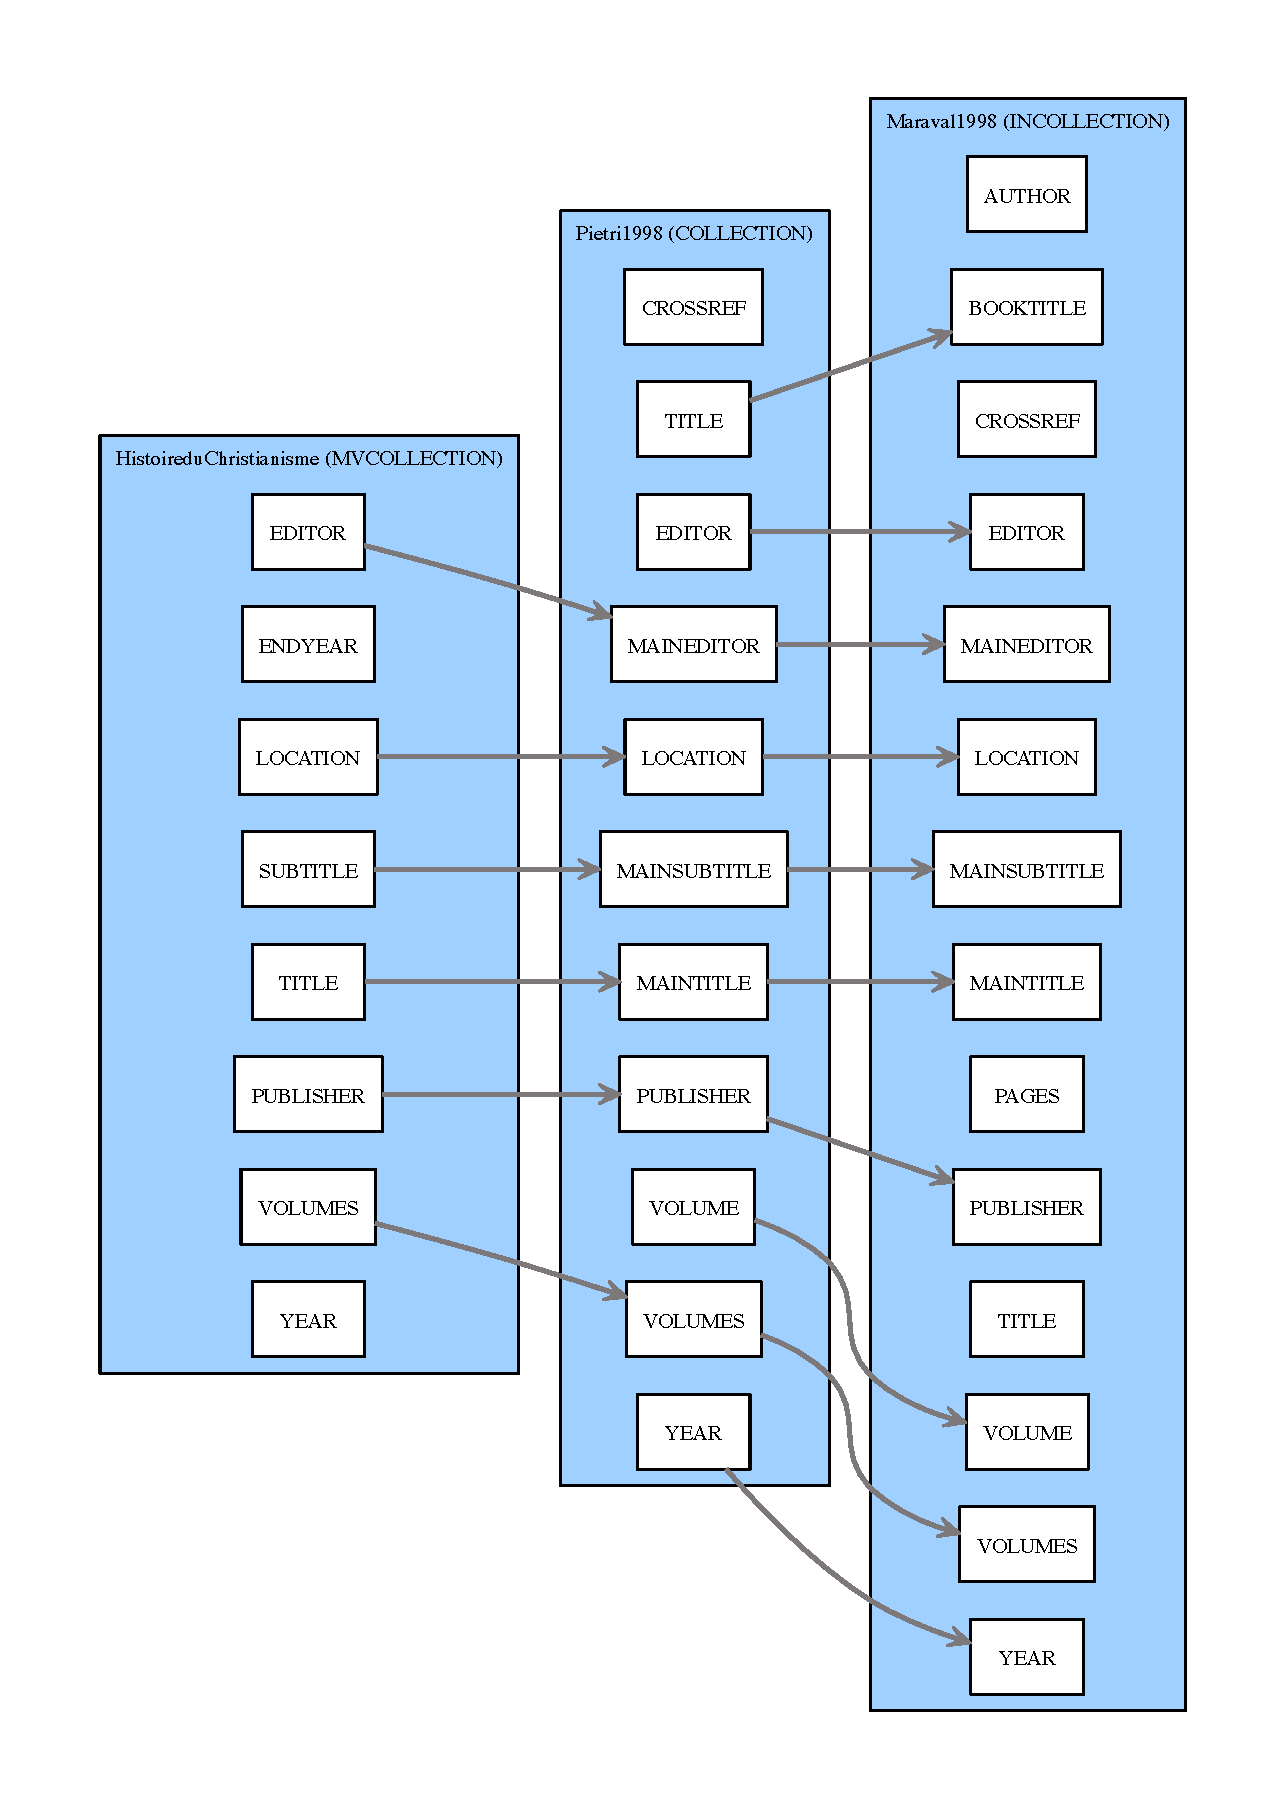
\includegraphics[height=0.99\textheight]{example-maineditor.pdf}
  \label{example-maineditor}
  \caption{Inheritance related to the \bibtype{maineditor} field}
\end{figure}
\subsubsection{Output example}

\begin{quotation}
\cite{HistoireduChristianisme}

\cite{Pietri1998}

\cite{Maraval1998}
\end{quotation}

\subsection{\bibfield{ineditor} and \bibfield{bookineditor}}
\subsubsection{Meaning}
For a \bibtype{article} or a \bibtype{inbook} entry, \bibfield{ineditor} means the editor of the single contribution, while \bibfield{editor} means the editor of the global volume.


For a \bibtype{bookinbook}, \bibfield{bookineditor} means the editor of the (ancient) edited book, while \bibfield{editor} means the editor of the global volume.

The \bibtype{ineditor} or the \bibfield{bookineditor} field is typeset immediately   after the title of the subentry, while the \bibtype{editor} field is typeset after the title of the main entry.

 


Notes that if the value of \bibtype{bookineditor} or \bibfield{ineditor} field is equal to the \bibfield{editor} field, this last one is not printed.

There is two modes of inheritance for these fields:  the default one and the optional one.

\subsubsection{Default inheritance mode}

With the default inheritance mode, the \bibtype{bookineditor} field of the subentry is never inherited from the main entry.
 

\paragraph{.bib example}

\inputminted[breaklines]{latex}{example-bookineditor.bib}

\paragraph{Fields inheritance}

The graph~\ref{example-bookineditor} shows the fields inheritance.

\begin{figure}
  \centering
  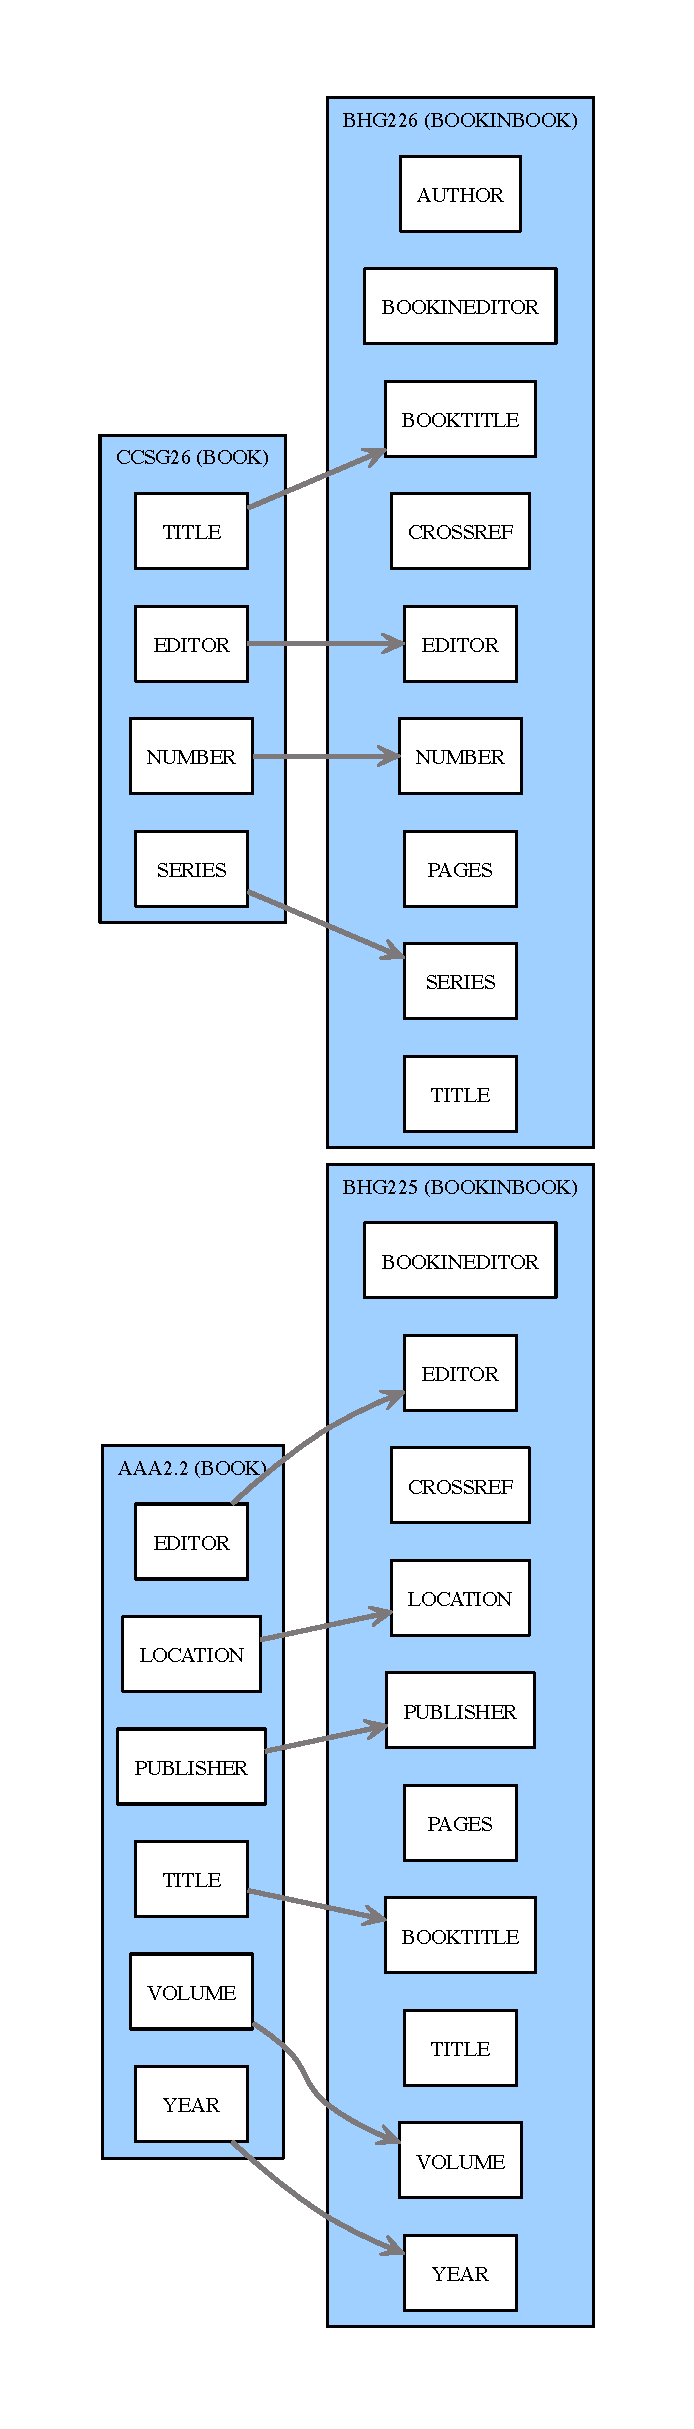
\includegraphics[height=0.99\textheight]{example-bookineditor.pdf}
  \label{example-bookineditor}
  \caption{Inheritance related to the \bibtype{bookineditor} field, default setting}
\end{figure}

 
\paragraph{Output example}

\begin{quotation}
  \cite{BHG226}
  
  \cite{BHG225}
\end{quotation}
\subsubsection{Optional inheritance}

With the optional inheritance, the \bibfield{bookineditor} or \bibfield{ineditor} field of the subentry is inherited from the \bibfield{editor} field of the main entry, except if the subentrty has already a \bibfield{bookineditor} or \bibfield{ineditor} field.


To enable this feature for the \bibfield{bookineditor} field, just add in your preamble, after loading biblatex, the following line:
\begin{minted}{latex}
\toggletrue{BookineditorFromEditor}
\end{minted}

To enable this feature for the \bibfield{ineditor} field, just add in your preamble, after loading biblatex, the following line:
\begin{minted}{latex}
\toggletrue{IneditorFromEditor}
\end{minted}

You can disable these features for specific subentry using \verb+noinherit=bookineditor+ or \verb`noinherit=ineditor` in the \bibfield{options} field of this subentry.

\paragraph{.bib example}

\inputminted[breaklines]{latex}{example-bookineditor-BookineditorFromEditor.bib}

\paragraph{Fields inheritance}

The graph~\ref{example-bookineditor-BookineditorFromEditor} shows the fields inheritance.

\begin{figure}
  \centering
  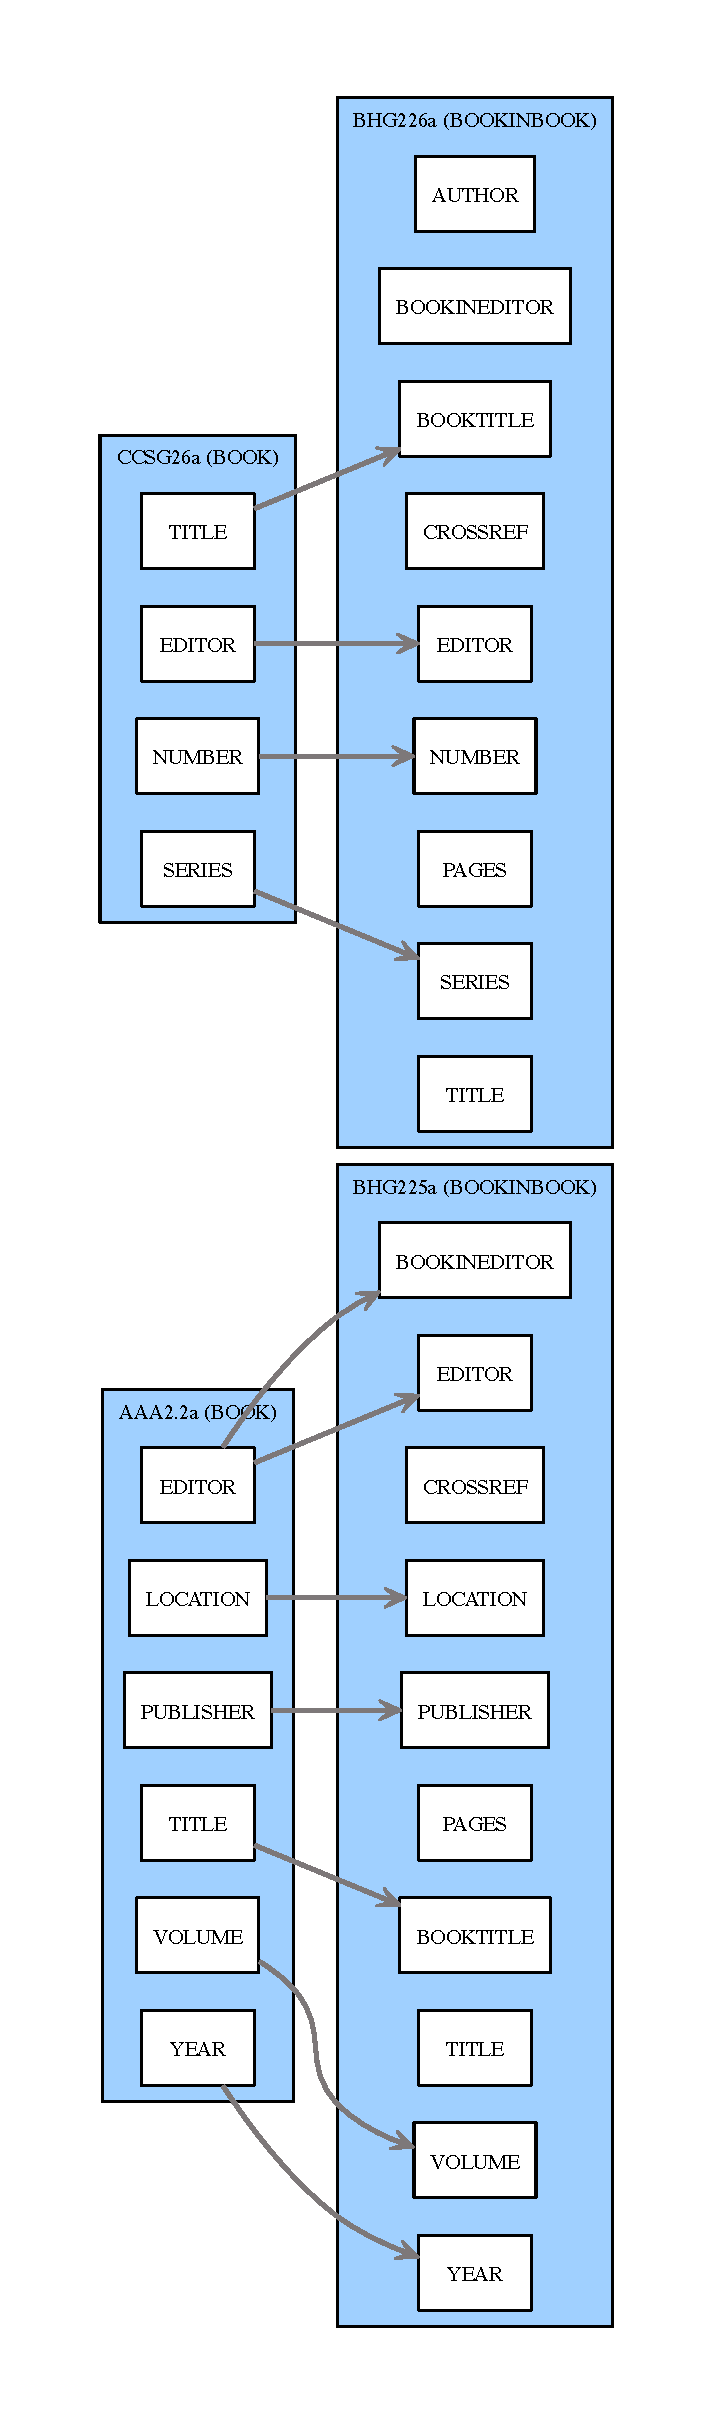
\includegraphics[height=0.99\textheight]{example-bookineditor-BookineditorFromEditor.pdf}
  \label{example-bookineditor-BookineditorFromEditor}
  \caption{Inheritance related to the \bibtype{bookineditor} field with optional inheritance}
\end{figure}

 
\paragraph{Output example}

\begin{quotation}
  \cite{BHG226a}
  
  \cite{BHG225a}
\end{quotation}
\section{Change history}
\begin{changelog}


\begin{release}{1.3.1}{2017-01-25}
  \item Fix spurious space when a book have nore author, nore editor.
\end{release}

\begin{release}{1.3.0a}{2016-11-26}
  \item Fix typo in handbook.
\end{release}

\begin{release}{1.3.0}{2016-11-23}
  \item Add \verb+noinherit=bookineditor+ and \verb+noinherit=ineditor+ options for individual volume.
\end{release}

\begin{release}{1.2.0}{2016-09-08}
  \item If the \bibfield{bookineditor} or \bibfield{ineditor} field is equal to the\bibfield{editor} field, the last one is not printed.
  \item Add two options to make \bibfield{bookineditor} or \bibfield{ineditor} to be inherited from  \bibfield{editor} field.
\end{release}

\begin{release}{1.1.1}{2016-09-07}
  \item Don't define again \verb+bybookineditor+ macro if already defined by \emph{biblatex-bookinother}.
\end{release}


\begin{release}{1.1.0}{2016-06-07}
  \item Add error message to know more quickly break compatibility with new releases of biblatex.
\end{release}

\begin{release}{1.0.0}{2016-04-06}
\item First public release.
\end{release}
\end{changelog}
\end{document}
